\documentclass{report}
\usepackage[francais]{babel}
\usepackage[T1]{fontenc}
\usepackage[utf8]{inputenc}
\usepackage{titlesec}
\usepackage{minted}
\usepackage{graphicx}

\usepackage[top=3.0cm]{geometry}
\usepackage{color}
\definecolor{grey}{rgb}{0.99,0.99,0.99}
\titleformat{\chapter}[hang]{\bf\huge}{\thechapter}{2pc}{}

\setcounter{secnumdepth}{3}
\setcounter{tocdepth}{3}
        
\begin{document}

\begin{titlepage}
\begin{center}
\end{center}

\flushright
\begin{center}
\bigskip
\bigskip
\bigskip
\bigskip
\bigskip
\bigskip
\bigskip
\bigskip
\bigskip
\bigskip
\bigskip
\bigskip
\huge{Projet de compilation: Transformation de données JSON}\\
\end{center}
\begin{center}
\bigskip
\bigskip
\bigskip
\bigskip
\bigskip
\bigskip
\bigskip
\bigskip
\bigskip
Romain Beaumont et Ru Jia\\
\bigskip
\bigskip
\bigskip
\bigskip
\bigskip
\bigskip
\bigskip
\bigskip
\bigskip
\bigskip
\bigskip
\bigskip
\bigskip
\bigskip
\bigskip

\textbf{du} 4 Décembre 2012  \textbf{au} 7 Janvier 2013

\bigskip
\bigskip
\bigskip
\end{center}
\end{titlepage}
 
\tableofcontents


\chapter{Introduction}
\par
L'objectif de ce projet est, en utilisant les outils ocamlyacc et ocamllex, de convertir du JSON en un arbre de syntaxe abstrait. Puis de convertir cet arbre en JSON, en XML et en SQL. Nous avons choisi de faire ce projet en ocaml car ce langage est adapté ici.

\chapter{Description de json}
\par
Le format JSON est une valeur.

\section{Valeur}
Une valeur peut être une chaîne de caractère, un nombre flottant, un objet, un tableau, true, false ou null.
\\
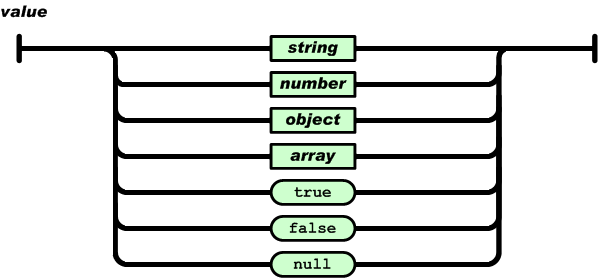
\includegraphics[width=8cm]{value.png}

\section{Objet}
Un objet est composé d’une liste de couples chaîne de caractère : valeur, séparés par des virgules, le tout entre accolades.
\\
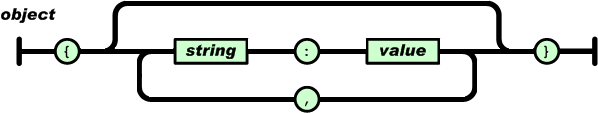
\includegraphics[width=8cm]{object.png}

\section{Tableau}
Un tableau est une liste de valeurs séparées par des virgules, le tout entre crochets.
\\
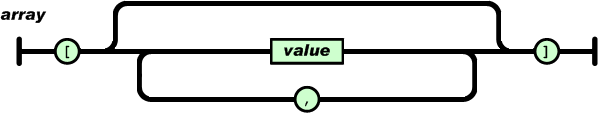
\includegraphics[width=8cm]{array.png}

\section{Chaine de caractère}
Une chaîne de caractère est composée d’une suite composée de caractères quelconques sauf " et $\backslash$  ou de $\backslash$  suivi de " $\backslash$  / b f n r t ou u ; le tout entre guillemets droits doubles (").
\\
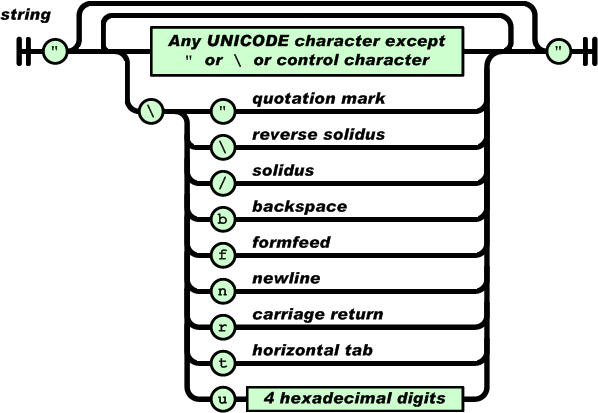
\includegraphics[width=8cm]{string.png}

\section{Nombre flottant}
Un nombre flottant est composé d’un signe - optionnel, d’un entier sans 0 non significatifs, suivi optionnellement d’une partie fractionnelle composée d’un point et d’un entier, et optionnellement d’un exposant composé d’un e en minuscule ou majuscule, d’un signe + ou - éventuel, et d’un entier.
\\
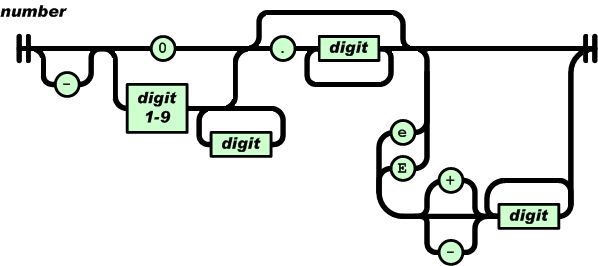
\includegraphics[width=8cm]{number.png}

\section{Exemple}
\begin{minted}[fontsize=\scriptsize,bgcolor=grey]{json}
[{ "string" : "chaine", "number" : 3.14e-2, 
   "bool" : true },
 { "bool" : false, "number" : null }]
\end{minted}



\chapter{Front end json}
L'objectif du front end json est de transformer une chaine de caractère contenant un format json en un arbre de syntaxe abstrait en ocaml. Pour cela il faut définir les types servant à stocker cette arbre de syntaxe abstraite, puis réaliser un lexeur puis un parseur.
\section{Types}
\par
Pour représenter un arbre de syntaxe abstraite json il nous a fallu définir des types ocaml. Nous avons donc défini 3 types : un type jvalue correspond à une valeur, un type jobject correspond à un objet et un type jarray correspondant à un tableau.
\par
Un tableau est une liste ordonné de valeur, nous avons donc choisi une jvalue list.
\par
Un objet est une liste de couple chaine de caractère, jvalue. On peut lire dans la RFC qu'à une chaine on associe toujours une unique jvalue. Nous avons donc choisi le type StringMap.t défini à partir de Map.Make (String) pour vérifier cette unicité.
\par
Pour le type valeur nous avons choisi un type somme afin de représenter les différentes choses qu'une valeur peut être.
\par
\begin{minted}[fontsize=\scriptsize,bgcolor=grey]{ocaml}
module StringMap = Map.Make (String);;

type jobject=jvalue StringMap.t
and jvalue=S of string|F of float|B of bool|N|O of jobject|A of jarray
and jarray=jvalue list;;
\end{minted}

\section{Lexer}
\par
Nous avons choisi d'utiliser String.sub s 1 ((String.length s)-2) pour enlever les quote avant et après la chaine.
\\
\begin{minted}[fontsize=\scriptsize,bgcolor=grey]{ocaml}
{open Parser}
rule token = parse
	[' ' '\r' '\t' '\n']     { token lexbuf }     (* skip blanks *)
	| ':'            { DP }
	| '{'	         { LEFTP}
	| '}'	         { RIGHTP}
	| '['	         { LEFTC}
	| ']'	         { RIGHTC}
	| ','	         {COMMA}
	| "false"         { FALSE }
	| "true"		{ TRUE }
	| "null"	     {NULL}
	| '-'?(['1'-'9']['0'-'9']*|'0')('.'['0'-'9']+)?(['e''E']['+''-']?['0'-'9']+)? 
	as f {FLOAT(float_of_string(f))}
	| '"'([^'"' '\\']|('\\'['"' '\\' '/' 'b' 'f' 'n' 'r' 't' 'u']))*'"' 
	as s  { STRING(String.sub s 1 ((String.length s)-2)) }
	| eof            { EOF }
\end{minted}

\section{Parser}
\par
Dans ce parseur on commence par définir les types et les token. On dit que le type attendu dans le main est une jvalue. puis on défini des expressions correspondantes aux types ocaml : jvalue,jarray,jobject. Pour jarray et jobject on a besoin de définir 2 autres expressions : liste\_jvalue et liste\_jobject\_value. Dans liste\_jobject\_value on vérifie qu'il y a bien unicite avant d'ajouter dans l'objet.
\\
\begin{minted}[fontsize=\scriptsize,bgcolor=grey]{ocaml}
%{open Type;;
exception Pas_unicite;;%}
%token TRUE FALSE NULL
%token <string> STRING
%token <float> FLOAT
%token LEFTP RIGHTP
%token LEFTC RIGHTC
%token COMMA DP
%token EOF
%start main
%type <Type.jvalue> main
%%


main:jvalue EOF {$1};

jarray:LEFTC liste_jvalue RIGHTC {$2};

liste_jvalue:
	jvalue COMMA liste_jvalue {$1::$3}
	| jvalue	 { $1::[] }
	| {[]}
	;

jvalue:
	TRUE {B true}
	|FALSE {B false}
	| STRING {S $1}
	| jobject {O $1}
	| jarray {A $1}
	|NULL {N}
	|FLOAT {F $1}
;

jobject:LEFTP liste_jobject_value RIGHTP {$2};

liste_jobject_value:
	STRING DP jvalue COMMA liste_jobject_value 
	{ if StringMap.mem $1 $5 then raise Pas_unicite else StringMap.add $1 $3 $5 }
	| STRING DP jvalue	 { StringMap.add $1 $3 (StringMap.empty) }
	| {StringMap.empty}
;
\end{minted}


\chapter{Back end}
\section{JSON}
\par
Dans cette partie on doit retransformer l'arbre de syntaxe abstraite en json. Cela permet de vérifier qu'on a bien traduit le json en arbre de syntaxe abstraite.

\par
Pour cela on ouvre le module Parser et Type puis on défini 3 fonctions : json\_string\_of\_jarray, json\_string\_of\_jobject et json\_string\_of\_jvalue qui retransforment respectivement les jarray, les jobject et les jvalue. Nous avons utilisé la fonction String.concat qui permet de transformer une liste en un chaine de caractère grâce à un séparateur. Pour les jarray nous avons utilisé la fonction List.map et pour les object la fonction StringMap.fold. jvalue est un simple type somme nous avons donc utilisé un match.

\par
Une fois la jvalue convertit en String il suffit de l'afficher avec print\_string.

\par
Ce fichier json\_to\_json.ml permet ainsi de former l'exécutable json\_to\_json.
\\
\begin{minted}[fontsize=\scriptsize,bgcolor=grey]{ocaml}
open Type;;
open Parser;;

let rec json_string_of_jarray a = 
"["^(String.concat "," (List.map json_string_of_jvalue a))^"]"
	
and json_string_of_jobject o ="{"^(String.concat "," 
(StringMap.fold 
(fun s jval l -> ("\""^s^"\""^":"^(json_string_of_jvalue jval))::l) o []))^"}"
	
and json_string_of_jvalue jval = match jval with
	| S s -> "\""^s^"\""
	| F f -> string_of_float f
	| B b -> (if b then "true" else "false")
	| N -> "NULL"
	| O jobj -> json_string_of_jobject jobj
	| A jarr -> json_string_of_jarray jarr;;
	
let pretty_print a=print_string (json_string_of_jvalue a);;

pretty_print (Parser.main Lexer.token (Lexing.from_channel stdin));;
print_newline();;
print_newline();;
\end{minted}
On peut vérifier que tous les exemples fonctionnent.

\section{XML}
\par
La conversion en XML est très similaire à celle en JSON. Néanmoins quelques différences : nous avons créé une fonction smap afin de créer la fonction stringUnderscoreOfSpace qui va transformer les espaces en underscore dans les string. Ensuite nous avons réalisé les fonctions xml\_string\_of\_jarray, xml\_string\_of\_jobject et xml\_string\_of\_jvalue très ressemblantes à celle pour JSON.
\\
\begin{minted}[fontsize=\scriptsize,bgcolor=grey]{ocaml}
open Type;;
open Parser;;

let smap f s = 
	let rec aux f s i =
		if i=(String.length s)-1 then s
		else (let _ =  s.[i]<- (f (s.[i])) in aux f s (i+1))
	in aux f s 0;;
	
let stringUnderscoreOfSpace s=smap (fun a -> if a = ' ' then '_' else a) s;;

let rec xml_string_of_jarray a = "<tab>"^(String.concat "" 
(List.map (fun jval -> "<item>"^(xml_string_of_jvalue jval)^"</item>") a))^"</tab>"
	
and xml_string_of_jobject o = String.concat "" (StringMap.fold 
(fun s jval l ->let t = stringUnderscoreOfSpace s  in  
("<"^t^">"^(xml_string_of_jvalue jval)^"</"^t^">")::l ) o [])
	
and xml_string_of_jvalue jval = match jval with
	| S s -> s
	| F f -> string_of_float f
	| B b -> (if b then "<true/>" else "<false/>")
	| N -> "<null/>"
	| O jobj -> xml_string_of_jobject jobj
	| A jarr -> xml_string_of_jarray jarr;;
	
	
let pretty_print a=print_string (xml_string_of_jvalue a);;

pretty_print (Parser.main Lexer.token (Lexing.from_channel stdin));;
print_newline();;
\end{minted}

Exemple : xml correpondant à first.json
\\
\begin{minted}[fontsize=\scriptsize,bgcolor=grey]{xml}
<tab><item><string>chaine</string><number>0.0314</number><bool><true/>
</bool></item><item><number><null/></number><bool><false/></bool></item></tab>
\end{minted}

\section{SQL}
\subsection{Inférence de type}
\par
A partir de jvalue on veut obtenir un jvalue type, voilà les types que nous avons défini pour atteindre cet objectif :
\\
\begin{minted}[fontsize=\scriptsize,bgcolor=grey]{ocaml}
module StringMap = Map.Make (String);;

type jvalue_type=TNull|TString|TNumber|TBool|TArray of jarray_type|TObject of jobject_type
and jobject_type=jvalue_type StringMap.t
and jarray_type=Ar of jvalue_type | V;;

type json_type=jvalue_type;;
\end{minted}
Pour jvalue\_type, on reprend la forme d'une jvalue mais sans les paramètres des constructeurs sauf pour les array et les object. Pour jobject\_type on utilise une StringMap comme pour les jobject. Pour jarray\_type on se rend compte que la fusion opéré sur les éléments d'un jarray pour produire un jarray\_type conduit au fait qu'un jarray\_type ne peut avoir que 0 ou 1 élement et on définit donc un type en conséquence.

\par
Une fois ces types définis dans infer\_type.ml on définis des fonctions qui vont fusionner les types : merge\_jobject\_type, merge\_jvalue\_type et merge\_jarray\_type. Pour jobject on va utiliser la fonction StringMap.merge. C'est dans merge\_jvalue\_type qu'on prend en compte que Null peut être remplacé par n'importe quel autre type.

\par
Nous avons ensuite fait 3 autre fonctions : infer\_jarray\_type, infer\_jobject\_type et infer\_jvalue\_type qui inférent les types en parcourant les variables initiales.

\par
Pour vérifier que l'inférence de type était bien réalisée nous avons ensuite fait quelques fonctions qui permettent d'afficher ces types comme dans l'exemple du sujet. Ainsi nous avons créé un exécutable json\_to\_type.

Exemple : type correspondant à first.json :
\\
\begin{minted}[fontsize=\scriptsize,bgcolor=grey]{ocaml}
Array(Object({("string",String);("number",Number);("bool",Bool)}))
\end{minted}

\subsection{Table}
\par
Dans un fichier json\_to\_sql.ml nous avons commencé par définir un type d'association qui va associer les json\_type à des noms c'est à dire des String. En réalité nous avons ensuite rendu ce type plus complexe pour rendre compte d'informations aussi nécéssaires. Ainsi un nom est composé d'un int et d'un string afin d'augmenter de faire des tables table1 table2 table3 si table existe déjà. Et nous avons adjoint à cette association un int StringMap.t pour savoir qu'elle était la plus grande valeur associée à une table (par exemple 3 à "table" ici)

\begin{minted}[fontsize=\scriptsize,bgcolor=grey]{ocaml}
module JsonTypeMap = Map.Make (struct
    type t = json_type
    let compare = Pervasives.compare
  end);;

type associationTypeTable=((int StringMap.t)*((string*int) JsonTypeMap.t));;

let emptyAssociationTypeTable=((StringMap.empty),(JsonTypeMap.empty));;
\end{minted}

Nous avons ensuite défini un type table et une fonction table\_string\_of\_table qui transforme ce type en un string contenant un create table.
\\
\begin{minted}[fontsize=\scriptsize,bgcolor=grey]{ocaml}
type table=string*((string*string) list);;
let table_string_of_table (nomTable,listeAttributs)=
	"create table "^nomTable^"\n"^
	"(\n"^(String.concat ",\n" (List.map (fun (nomAttribut,typeAttribut) ->
	(stringUnderscoreOfSpace nomAttribut)^" "^typeAttribut) listeAttributs))^"\n);\n";;
\end{minted}

Pour obtenir ce type table nous avons fait d'autres fonctions : table\_of\_jobject\_type, table\_of\_jarray\_type et table\_of\_jvalue\_type qui font ce que leurs noms indiquent.
Grâce à ces fonctions nous avons ensuite réalisé find\_table\_of\_type.

\subsection{Insert}
\par
Pour cette partie nous avons fait une fonction string\_of\_insert qui permet grâce à quelques informations de générer la string correpondant à un insert into.
\\
\begin{minted}[fontsize=\scriptsize,bgcolor=grey]{ocaml}
let string_of_insert nomTable id listeNom listeValeur=
	"insert into "^(nomTable)^" ("^(String.concat "," (((nomTable)^"_idx")::listeNom))^")\n"^
	"values("^(String.concat "," ((string_of_int id)::listeValeur))^");\n";;
\end{minted}
Nous avons ensuite appelé cette fonction ainsi que find\_table\_of\_type pour créer les fonctions insert\_sql\_string\_of\_jvalue, insert\_sql\_string\_of\_jobject et insert\_sql\_string\_of\_jarray.
\par
Une fois cela fait nous avons put appelé infer\_type et insert\_value pour générer l'exécutable json\_to\_sql.
\subsection{Exemples}
Sql correpondant à first.json :
\\
\begin{minted}[fontsize=\scriptsize,bgcolor=grey]{sql}
create table main
(
main_idx INT,
string TEXT,
number FLOAT,
bool INT
);
insert into main (main_idx,number,bool)
values(2,NULL,0);
insert into main (main_idx,string,number,bool)
values(1,"chaine",0.0314,1);
\end{minted}

Le nom de la table est main dans ce cas :\\
test6.json :
\\
\begin{minted}[fontsize=\scriptsize,bgcolor=grey]{json}
["t1","t2","t3","t4"]
\end{minted}

Sql correspondant :
\\
\begin{minted}[fontsize=\scriptsize,bgcolor=grey]{sql}
create table main                                                                                                                                                      
(                                                                                                                                                                      
main_idx INT,                                                                                                                                                          
mainA TEXT                                                                                                                                                             
);                                                                                                                                                                     
insert into main (main_idx,mainA)                                                                                                                                      
values(4,"t4");                                                                                                                                                        
insert into main (main_idx,mainA)
values(3,"t3");
insert into main (main_idx,mainA)
values(2,"t2");
insert into main (main_idx,mainA)
values(1,"t1");
\end{minted}

Dans ce genre de cas on incrémente le numéro de la table :\\
test9.json :
\\
\begin{minted}[fontsize=\scriptsize,bgcolor=grey]{json}
[[1,2],[3,4]]
\end{minted}

Sql correspondant :
\\
\begin{minted}[fontsize=\scriptsize,bgcolor=grey]{sql}
create table main
(
main_idx INT,
main1_begin INT,
main1_end INT
);
create table main1
(
main1_idx INT,
mainA FLOAT
);
insert into main1 (main1_idx,mainA)
values(6,4.);
insert into main1 (main1_idx,mainA)
values(5,3.);
insert into main (main_idx,main1_begin,main1_end)
values(4,5,6);
insert into main1 (main1_idx,mainA)
values(3,2.);
insert into main1 (main1_idx,mainA)
values(2,1.);
insert into main (main_idx,main1_begin,main1_end)
values(1,2,3);
\end{minted}

Mais dans ce genre de cas on conserve le nom des attributs même s'ils ne peuvent pas correpondrent avec le nom de la table (on laisse le soin à l'utilisateur de ces tables de s'y retrouver) :\\
test7.json :
\\
\begin{minted}[fontsize=\scriptsize,bgcolor=grey]{json}
[{"el1":["1t1","1t2","1t3","1t4"],"el2":["2t1","2t2","2t3","2t4"]}]
\end{minted}

Sql correspondant :
\\
\begin{minted}[fontsize=\scriptsize,bgcolor=grey]{sql}
create table main
(
main_idx INT,
el2_begin INT,
el2_end INT,
el1_begin INT,
el1_end INT
);
create table el1
(
el1_idx INT,
mainA TEXT
);
insert into el1 (el1_idx,mainA)
values(4,"1t4");
insert into el1 (el1_idx,mainA)
values(3,"1t3");
insert into el1 (el1_idx,mainA)
values(2,"1t2");
insert into el1 (el1_idx,mainA)
values(1,"1t1");
insert into el1 (el1_idx,mainA)
values(8,"2t4");
insert into el1 (el1_idx,mainA)
values(7,"2t3");
insert into el1 (el1_idx,mainA)
values(6,"2t2");
insert into el1 (el1_idx,mainA)
values(5,"2t1");
insert into main (main_idx,el2_begin,el2_end,el1_begin,el1_end)
values(9,5,8,1,4);
\end{minted}

Voici un cas où il n'y a pas unicité dans le jobject (le json n'est donc pas valide d'après la RFC) :
test20.json :
\\
\begin{minted}[fontsize=\scriptsize,bgcolor=grey]{json}
{"la":5,"la":6,"lo":4}
\end{minted}
Cela renvoie Fatal error: exception Parser.Pas\_unicite

Les autres tests présents dans le dossier exemple fonctionnent eux aussi en testant des cas plus ou moins particuliers. Le fichier testfacebook.json présente un exemple d'application réélles : données tirées de l'api facebook graph.

\chapter{Makefile, dépendance, exécution, tests et documentation}
\par
Pour compiler ce projet nous avons réalisé un Makefile. Nous avons utilisé ocamlc, ocamllex et ocamlyacc. Nous avons utilisé la fonction merge des Map et il faut donc disposer de ocaml 3.12 au minimum pour compiler.
\par
Pour tester le projet il suffit donc de faire make puis par exemple bin/json\_to\_sql < exemple/first.json
\par
test.pl et validation.pl permettent de vérifier que les tests du sql donnent bien ce qui est attendu, très utile lors de modification du code de json\_to\_sql.pl. Les fichiers *.attentu.sql dans le dossier exemple sont les résultats attendus. On peut les générer avec validation.pl lorsqu'on est sûr que json\_to\_sql fonctionne bien.
\par
sqltopsql.pl permet de rendre le code sql généré utilisable par postgresql (transformation des " en ' et ajout de begin; et commit;)
\par
On peut aussi faire make clean et make test\_to\_xml
\par
En faisant make htmldoc on peut générer une documentation grâce à ocamldoc qui se trouvera dans le dossier htmldoc, commencer par htmldoc/index.html.


\chapter{Conclusion}
\section{Résultats}
Tout les exemples dans le dossier exemple fonctionnent que ce soit pour le json, le xml, les types ou le sql.
\section{Avancement personnel}
\par
Ce projet a permis d'apprendre à manipuler lex et yacc et de pratiquer le ocaml. Il peut être utilisé pour de nombreuses choses, par exemple pour transformer les données venant d'une api, par exemple celle de facebook.

\end{document}